%%%%%%%%%%%%%%%%%%%%%%%%%%%%%%%%%%%%%%%%%%%%%%%%%%%%%%%%%%%%%%%%%%%%
%% I, the copyright holder of this work, release this work into the
%% public domain. This applies worldwide. In some countries this may
%% not be legally possible; if so: I grant anyone the right to use
%% this work for any purpose, without any conditions, unless such
%% conditions are required by law.
%%%%%%%%%%%%%%%%%%%%%%%%%%%%%%%%%%%%%%%%%%%%%%%%%%%%%%%%%%%%%%%%%%%%

\documentclass[
  digital, %% This option enables the default options for the
           %% digital version of a document. Replace with `printed`
           %% to enable the default options for the printed version
           %% of a document.
  table,   %% Causes the coloring of tables. Replace with `notable`
           %% to restore plain tables.
  lof,     %% Prints the List of Figures. Replace with `nolof` to
           %% hide the List of Figures.
  lot,     %% Prints the List of Tables. Replace with `nolot` to
           %% hide the List of Tables.
  %% More options are listed in the user guide at
  %% <http://mirrors.ctan.org/macros/latex/contrib/fithesis/guide/mu/fi.pdf>.
  oneside
]{fithesis3}
%% The following section sets up the locales used in the thesis.
\usepackage{listings}
\usepackage[resetfonts]{cmap} %% We need to load the T2A font encoding
\usepackage[T1,T2A]{fontenc}  %% to use the Cyrillic fonts with Russian texts.
\usepackage[
  main=english, %% By using `czech` or `slovak` as the main locale
                %% instead of `english`, you can typeset the thesis
                %% in either Czech or Slovak, respectively.
 %english, german, russian, czech, slovak %% The additional keys allow
]{babel}        %% foreign texts to be typeset as follows:
%%
%%   \begin{otherlanguage}{german}  ... \end{otherlanguage}
%%   \begin{otherlanguage}{russian} ... \end{otherlanguage}
%%   \begin{otherlanguage}{czech}   ... \end{otherlanguage}
%%   \begin{otherlanguage}{slovak}  ... \end{otherlanguage}
%%
%% For non-Latin scripts, it may be necessary to load additional
%% fonts:
\usepackage{paratype}

\usepackage[
   backend=biber        % if we want unicode
  ,style=authoryear % or iso-numeric for numeric citation method
  ,autolang=other       % to support multiple languages in bibliography
  ,sortlocale=cs_CZ     % locale of main language, for sorting
  ,bibencoding=UTF8     % this is necessary only if bibliography file is in different encoding than main document
]{biblatex}
\def\textrussian#1{{\usefont{T2A}{PTSerif-TLF}{m}{rm}#1}}
%%
%% The following section sets up the metadata of the thesis.
\thesissetup{
    date          = \the\year/\the\month/\the\day,
    university    = mu,
    faculty       = fi,
    type          = mgr,
    author        = Tomáš Šíma,
    gender        = m,
    advisor       = {RNDr. Martin Stehlík, Ph.D, Mgr. Jaroslav Šeděnka},
    title         = {OSINT: Correlation and inference of information from social media},
    TeXtitle      = {OSINT: Correlation and inference of information from social media},
    keywords      = {blockhain, bitcoin, OSINT, darkweb, drug market, TOR, cryptocurrency, anonymity, metadata},
    TeXkeywords   = {blockhain, bitcoin, OSINT, darkweb, drug market, TOR, cryptocurrency, anonymity, metadata},
    abstract      = {The goal of this thesis is to create a tool to find, analyze and visualize publicly available data, which can be helpful to deanonymize users of drug markets available via TOR on dark web. The aim of this tool is to help investigators with collecting intelligence on entities related to these drug markets. Users and operators of these markets employ multiple means to prevent their deanonymization. The markets are operated ad TOR services, PGP encryption is often required to use in communication between multiple parties and bitcoin is used as a way to pay for goods or services.
    
    We scraped multiple publicly available social sites and websites related to bitcoin(twitter,bitcointalk, reddit, blockchain.info...) and drug markets thereself using python. Westored all these data into AgensGraph database, which is a graph database based on PostgreSQL. Wecreated a tool, which uses these data and multiple heuristics to analyze and visualize data and metadata of users,drug markets, social media and blockchain. Tool can also for given adress find the nearest adresses or transactions related to drug markets and also find the nearest adresses that are mentioned in scraped websites. 
    
    To test the efficiency of this tool, we created multiple profiles on these dark markets and performed multiple transactions to deposit and withdraw bitcoins. The tool identified these and these percent of transactions.
    },
    thanks        = {I would like to thank my supervisor RNDr. Martin Stehlík Ph.D for guiding me and providing technical support for my work. 
    
    I would also like to thank Mgr. Jaroslav Šeděnka for his continuous stream of helpful comments and ideas.
    
    Access to computing and storage facilities owned by parties and projects contributing to the National Grid Infrastructure MetaCentrum provided under the programme "Projects of Large Research, Development, and Innovations Infrastructures" (CESNET LM2015042), is greatly appreciated.},
    bib           = citations.bib
}

\usepackage{makeidx}      %% The `makeidx` package contains
\makeindex                %% helper commands for index typesetting.
%% These additional packages are used within the document:
\usepackage{paralist} %% Compact list environments
\usepackage{amsmath}  %% Mathematics
\usepackage{amsthm}
\usepackage{amsfonts}
\usepackage{url}      %% Hyperlinks
\usepackage{markdown} %% Lightweight markup
\usepackage{listings} %% Source code highlighting
\usepackage{graphicx}
\graphicspath{ {images/} }
\lstset{
  basicstyle      = \ttfamily,%
  identifierstyle = \color{black},%
  keywordstyle    = \color{blue},%
  keywordstyle    = {[2]\color{cyan}},%
  keywordstyle    = {[3]\color{olive}},%
  stringstyle     = \color{teal},%
  commentstyle    = \itshape\color{magenta}}
\usepackage{floatrow} %% Putting captions above tables
\floatsetup[table]{capposition=top}
\begin{document}
\chapter{Introduction}
%\addcontentsline{toc}{chapter}{Introduction}

The relative anonymity of internet offer an incentive for criminal parties to use internet as a tool for their activities.
Internet facilitated some forms of existing crimes(Selling drugs and guns, counterfeits selling, Ponzi schemes) and also enabled many new types of frauds like hacking, phishing and carding.
Police statistics show, that crime happening online is much less likely to be discovered and criminals persecuted. Criminals value their anonymity very high and use various means to make them even more anonymous,
like VPNs and TOR. The big problem for criminals were getting the money they got from criminal activity to their possession(In banknotes, or to their bank account), since that requires some form physical presence.
Also, it was hard for two anonymous entities engaging in criminal activity to transfer money to each other, since none could be sure about the origin of money they are receiving.

For bitcoin, there is no central authority requiring bitcoin address( bitcoin equivalent of bank account number) to be linked to person's identity.
Criminals can use their anonymous connection to internet to both recieve and send bitcoins and therefore not disclose their identity.
This feature of bitcoin and other cryptocurrencies gave rise to drug markets, which can be publicly accessed via TOR. However,
the history of all bitcoin transactions is publicly available and so each bitcoin can be tracked through the whole transaction history.

In this work we collect multiple public sources of data about bitcoin transactions, bitcoin adresses and drug markets.
We examine these data in order to describe the behaviour of drug markets users (distribution of sellers, availability of drugs,
number of users, revenues) and also to see, if these data can be used for disclosing identity of users and operators of drug markets.

\section{Goals}

The main goal of this thesis is to map two currently available drug markets 
and try multiple approaches for deanonymization of identities related to these drug markets.
Another outcome of this work is a proof of concept tool, that uses the data mentioned above to help investigator to disclose transactions,
addresses and identities related to online drug markets.
The secondary outcome of this work is gathering data about the trades, which happened on the drug markets and
 gather interesting statistics about the whole market as well as actors operating there.

\section{Structure of thesis}

The following text describes individual chapters forming structure of this thesis.
The chapter Related works give overview of work already done on similar topics and 
how this work differ or extend the previous done research.

The chapter Technology and terms gives quick introduction to bitcoin and blockchain, which is used for paying on crypto markets.
Then it describes how the dark markets operate within dark web.

The chapter Methods and tools to get and analyze data describe the proccess of collecting the data from bitcoin blockchain,
drug markets and pubicly available sites(Mainly forums and social networks). 

The Deanonymization techniques chapter descibe heuristics and methods that are later used by the proof of concept application to detect 
addresses used by drug markets and link the users of drug markets to publicly found identities.

The chapter Statistics of drug markets describes various statistics about drug markets, that were gathered during drug market website scraping.
It contains two parts, the first is focused on statistics related to money, the second part is giving insight about non-money related statistics.

POC application chapter describes the functionality, implementation and 
possible future development of application for investigating bitcoin addresses, which was created as part of this thesis.

Testing and verification of the created tool descibes the proccess by which the proof of concept application was tested and the results

The last chapter Discussion is about achieving goals, problems of implementation and future work.

\chapter{Related works}
\section{Pairing blockchain transactions with public data}
Multiple papers were published regarding analysis of blockchain graph. The \parencite{reid2013analysis} was published in 2013 and dealt with much smaller number of people using bitcoin and smaller transaction graph.
Their analysis also focus on danonymization through multiple aspects of bitcoin protocol, while this thesis focus on deanonymization from transaction graph and public data.
The \parencite{ron2013quantitative} focus on bringing interesting statistics about bitcoin transaction graph and track only really big(>50000 BTC)
transactions on the network. The authors of this paper also had to deal with much smaller blockchain graph.

Similar work to this thesis was done by \parencite{fleder2015bitcoin}. This paper use data from bitcointalk, the most popular bitcoin forum. 
They apply simple algorithm to group multiple bitcoin adresses belonging to one user together. Than they use the scraped data to show
that some of the bitcointalk users were using silkroad marketplace or other popular services accepting bitcoin.

Advanced and similar work was done by \parencite{spagnuolo2014bitiodine}. They downloaded the blockchain, transformed to the database
and performed clustering to get graph of transaction between users.
Than they developed a tool, which scraped data from multiple locations(bitcointalk and bitcoin-OTC forum) to link off-chain data and identities to bitcoin adresses.
They tested the tool on few popular transactions related to seizure of silkroad marketplace.

All of the previously mentioned works had to deal with much smaller transaction graph, as the usage of bitcoin grew exponentionally over the last year. 
My work is unique in that way, that it utilize much more sources of data, than the works previous mentioned. Also, the aim of this tool is to be able
to identify even just regular users of drug markets, not just big and important transactions.

\section{Behaviour of drug markets users and operators}

Papers describing the drug market users,vendors and the dynamic of
the online drug marketplace economy mostly focused on data related to silkroad marketplace seizure. 
Few authors described, how is the whole drug trafficking crime changing overtime with the coming of the new technologies.
There are only few articles focusing on describing the economy of fully operating drug market at the time of data collection.
In this work, we bring analysis of the micro-economy of two fully operating drug markets and present interesting statistics about vendors,
size and frequency of the deals and their sortiment and availability.

\chapter{Technology and terms}

In this chapter, I explain the terms, tools and related technology used for achieving the goal of this thesis.

\section{Bitcoin and blockchain}
Blockchain
For a broader coverage related to this topic, see Blockchain.

Number of unspent transaction outputs
The blockchain is a public ledger that records bitcoin transactions.
A novel solution accomplishes this without any trusted central authority: the maintenance of the blockchain is performed by a network of communicating nodes
running bitcoin software.Transactions of the form payer X sends Y bitcoins to payee Z are broadcast to this network using readily available software applications.
nodes can validate transactions, add them to their copy of the ledger, and then broadcast these ledger additions to other nodes. The blockchain is a distributed database – to achieve independent verification of the chain of ownership 
of any and every bitcoin amount, each network node stores its own copy of the blockchain. Approximately six times per hour, a new group of accepted transactions, a block, is created, added to the blockchain, and quickly published to all nodes.
This allows bitcoin software to determine when a particular bitcoin amount has been spent, which is necessary in order to prevent double-spending in an environment without central oversight. 
Whereas a conventional ledger records the transfers of actual bills or promissory notes that exist apart from it, the blockchain is the only place that bitcoins can be said to exist in the form of unspent outputs of transactions.

Transactions

Number of bitcoin transactions per month (logarithmic scale)
See also: Bitcoin network
Transactions are defined using a Forth-like scripting language.Transactions consist of one or more inputs and one or more outputs.
When a user sends bitcoins, the user designates each address and the amount of bitcoin being sent to that address in an output. 
To prevent double spending, each input must refer to a previous unspent output in the blockchain. The use of multiple inputs corresponds to the use of multiple coins in a cash transaction.
Since transactions can have multiple outputs, users can send bitcoins to multiple recipients in one transaction. As in a cash transaction, the sum of inputs (coins used to pay) can exceed the intended sum of payments.
In such a case, an additional output is used, returning the change back to the payer.Any input satoshis not accounted for in the transaction outputs become the transaction fee.

Privacy
Bitcoin is pseudonymous, meaning that funds are not tied to real-world entities but rather bitcoin addresses. Owners of bitcoin addresses are not explicitly identified, but all transactions on the blockchain are public. 
In addition, transactions can be linked to individuals and companies through "idioms of use" (e.g., transactions that spend coins from multiple inputs indicate that
the inputs may have a common owner) and corroborating public transaction data with known information on owners of certain addresses. Additionally, bitcoin exchanges, where bitcoins are traded for traditional
currencies, may be required by law to collect personal information.

To heighten financial privacy, a new bitcoin address can be generated for each transaction. For example, hierarchical deterministic wallets generate pseudorandom "rolling addresses"
for every transaction from a single seed, while only requiring a single passphrase to be remembered to recover all corresponding private keys. Researchers at Stanford University
and Concordia University have also shown that bitcoin exchanges and other entities can prove assets, liabilities, and solvency without revealing their addresses using zero-knowledge proofs.
"Bulletproofs," a version of Confidential Transactions proposed by Greg Maxwell, have been tested by Professor Dan Boneh of Stanford. Other solutions such Merkelized Abstract Syntax Trees (MAST),
pay-to-script-hash (P2SH) with MERKLE-BRANCH-VERIFY, and "Tail Call Execution Semantics, have also been proposed to support private smart contracts.


\section{TOR - the onion routing}
Tor is free software for enabling anonymous communication. The name is derived from an acronym for the original software project name "The Onion Router". 
Tor directs Internet traffic through a free, worldwide, volunteer overlay network consisting of more than seven thousand relays to conceal a user's location
and usage from anyone conducting network surveillance or traffic analysis. Using Tor makes it more difficult to trace Internet activity to the user: this includes 
"visits to Web sites, online posts, instant messages, and other communication forms". The intent for Tor's use is to protect the personal privacy of its users,
as well as their freedom and ability to conduct confidential communication by keeping their Internet activities from being monitored.

Tor does not prevent an online service from determining when it is being accessed through Tor. Tor protects a user's privacy,
but does not hide the fact that someone is using Tor. Some websites restrict allowances through Tor. For example, the MediaWiki TorBlock extension automatically restricts edits made through Tor,
although Wikipedia allows some limited editing in exceptional circumstances.

Onion routing is implemented by encryption in the application layer of a communication protocol stack, nested like the layers of an onion. 
Tor encrypts the data, including the next node destination IP address, multiple times and sends it through a virtual circuit comprising successive, random-selection Tor relays.
Each relay decrypts a layer of encryption to reveal the next relay in the circuit to pass the remaining encrypted data on to it. The final relay decrypts the innermost layer of encryption and sends
the original data to its destination without revealing or knowing the source IP address. Because the routing of the communication is partly concealed at every hop in the Tor circuit,
this method eliminates any single point at which the communicating peers can be determined through network surveillance that relies upon knowing its source and destination.

\section{Online drug marketplaces}
A darknet market or cryptomarket is a commercial website on the web that operates via darknets such as Tor or I2P
They function primarily as black markets, selling or brokering transactions involving drugs, cyber-arms, weapons,
counterfeit currency, stolen credit card details, forged documents, unlicensed pharmaceuticals, steroids and
other illicit goods as well as the sale of legal products. In December 2014, a study by Gareth Owen from the University
of Portsmouth suggested the second most popular sites on Tor were darknet markets.

Transactions typically use Bitcoin for payment, sometimes combined with tumblers for added anonymity and PGP to secure communications
between buyers and vendors from being stored on the site itself. Many sites use Bitcoin multisig transactions 
to improve security and reduce dependency on the site's escrow. The Helix Bitcoin tumbler offers direct anonymized marketplace payment integrations.

On making a purchase, the buyer must transfer cryptocurrency into the site's escrow, after which a vendor dispatches their goods then claims the
payment from the site. On receipt or non-receipt of the item users may leave feedback against the vendor's account. Buyers may "finalize early"
(FE), releasing funds from escrow to the vendor prior to receiving their goods in order to expedite a transaction, but leave themselves vulnerable to fraud if they choose to do so.

Following Operation Onymous, there was a substantial increase in PGP support from vendors, with PGP use on two marketplaces near 90\%.
This suggests that law enforcement responses to cryptomarkets result in continued security innovations, thereby making markets more resilient to undercover law enforcement efforts.

\chapter{Methods and tools to get and analyze data}
\section{Obtaining,storing and analyzing blockchain data}
In order to create a tool, that will find data related to bitcoin adresses, we need to store the blockchain locally in that way, that common graph algorithms can be applied.
We ran the official bitcoin daemon (further referenced as bitcoind), to obtain a copy of bitcoin blockchain. Bitcoind store blockchain in multiple *.blk files.
These files have structure, which is unfit for searching, processing and analysis of blockchain, so I used rusty-parser to parse these files and create csv files of transactions, outputs and adresses.

Than we imported these files into neo4j graph database, to have whole transaction graph in one place and be able to compute statistics and heuristics.
All entities in the \ref{neo4jschema} are represented as graph nodes, the relationships between them are edges.
\begin{figure}[!htb]
    \centering
    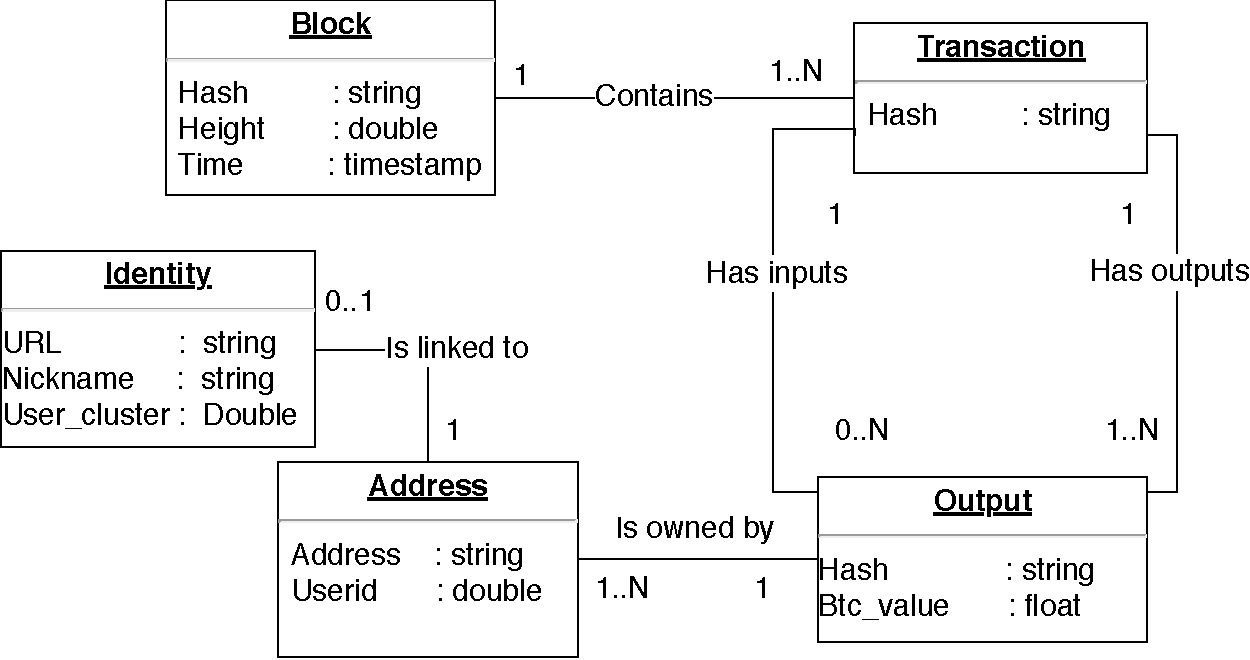
\includegraphics[width=1\textwidth]{neo4j-schema}
    \caption{Neo4j database ER diagram}
    \label{neo4jschema}
\end{figure}

\section{Drug markets web scraping and data collection}
We scraped data from dream market and valhalla, 2 big popular drug markets available via TOR. Wescraped the vendor nicknames, buyer reviews and the sortiment that each vendor sells.
We tested, if every transaction that is happening on drug market has its counter transaction in bitcoin blockchain. Wesent 0.05 bitcoins to both markets,
bought a virtually deliverable legally service(link to secret forum) and checked, if the bitcoins that I have sent to deposit adress left.
For both markets, there was no transaction happening for days after the transaction was done. This means, that markets don't transfer bitcoins,
when there is filled order, all the transactions that these drug markets do are just for depositing bitcoins on drug market account,
withdraw bitcoins and money laundering bitcoins.
We made multiple deposits and withdraws from drug markets in order to track, where were the deposited bitcoins transfered and where the withdrawn bitcoins originated.
These deposits and withdrawals are used to test the resulting application
We scraped 158 vendor PGP keys from dream market and 70 PGP keys from walhalla. Wetested these keys, if they are vulnerable to ROCA attack, via python module roca-detect. None of these keys were vulnerable.
All these PGP keys were searched for User-Id in metadata of PGP key and these user-Ids were seached by google. None of thesearches for user-Ids(both nicknames and mail addresses) returned any results.

We thought that metadata from the photos of drugs, which are available on the drug markets might be useful.
We downloaded hundreds of pictures both from walhalla and dream market.
Only metadata directly dependending on image content(like amount of red, green and blue colors) differ,
metadata that could potentionally help dislosing user identity(date of creation nad modification, signature, software version) were the same.
The software version contained line: $ImageMagick 6.8.9-9 Q16 x86_64 2017-07-31 http://www.imagemagick.org$
We created vendor account on both markets and uploaded an image with custom made metadata to see,
if the metadata were scraped and same version of software version appears. It happened so for both markets,
therefore we believe, that markets automatically scrape metadata from uploaded images in order to protect privacy of the users.

\section{Drug market server fingerprinting}
We tried to scan ports of drug markets servers and fingerprint their webserver, in order to find any vectors of further information gathering.
We scanned both drug markets servers using netcat, finding, that the only opened port is number 443(HTTPS), which is used by webserver.
We used httprecon to fingerprint used HTTP server. The fingerprinting consists of sending multiple malformed HTTP requests and comparing the webserver output with the database of responses by different webservers.
The results of fingerprinting can be see in figure xxx, the best matches are various modern versions of apache webserver.
The results of port scan and webserver printing doesn't indicate any way how to gather data about drug markets servers.

\section{Publicly available data scraping}
In order to have some bitcoind addresses and bitcoins linked to identities, We searched internet for pages, where are bitcoin adresses tied to real or virtual identities.
The interesting sites that I decided to scrape were bitcointalk forum, bitcoin-OTC, reddit, twitter, bitcoin.info.
The bitcointalk and bitcoin-OTC are the most popular internet forums related to cryptocurrencies. The script bitcointalk-scraper.py visits profile pages of all profiles on both forums (even those without any posts)
 and matched with bitcoin address regular expression.
 
The reddit and twitter were scraped by twitter-reddit-scraper.py. The script contain several hardcoded phrases like "Donate bitcoin" and "bitcoind address" and scrapes the results of search page.
Bitcoin.info is a webpage that serves primarly as bitcoin blockchain explorer, secundary,
it gathers multiple statistics about bitcoin blockchain and also offers for third parties to have their bitcoin address and identity listed on their webpage.
Some of these identities are verifies by signaturing custom made message with the bitcoin address associated private key.

We scraped data with the intention to link identities to bitcoin addresses. The data scraped from public sources are rows with thre collums: bitcoin addres, URL where was the addres scraped and username of the associated identity.
All data scraped from the public sources(bitcointalk, reddit,twitter, bitcoin-OTC) are imported to the same neo4j graph database as metadata belonging to the nodes representing given address.


\chapter{Deanonymization techniques}
\section{Detecting wallets owned by drug markets}
\section{Using own transactions to get market wallets}

\chapter{Statistics of drug markets}
Since we are trying to identify 


\section{Methodology}
The data was collected from walhalla drug market on 20.1.2018.
This url's of all market listings are in pattern http://valhallaxmn3fydu.onion/products/xxx where 
xxx is incrementing with each new listing.
We wrote a small script in bash to iterate through all the listings and download them using wget.
To be able to download via wget from .onion links, I had to use privoxy, to redirect the wget through locally ran TOR daemon.
After downloading all the pages of products, we parsed the downloaded files using python and common linux command 
line tools(cat,grep,cut,sed)
From the listing, we parsed vendor's nickname, the subcategory where the listing was placed and title of listing.

By this, we got 666 unique vendors name, so we downloaded and scraped the vendor's profiles pages from the walhalla 
market in similar way.
From the vendor's profile pages, we scraped name of vendor, his total revenue, number of positive and negative reviews 
and the countries from which the vendor ships.
The shortcoming of this method is, that we can download and analyze only sellers, 
that have at least one active listing at the time of data collection. 
Hovewer, we managed to download 20000 listings out of 100000.

The statistics, tables and plots in this chapter were produced by statistical and data analysis software R.
The exact commands to generate these figures and plots can be found in attachments in file named 'valhalla-r.txt'.

\section{Overall statistics of Walhalla drug market}

Walhalla was originally founded as local Finnish market,
that seems the reason for surprisingly many vendors shipping from Finland.
The reader can see the frequency of countries the vendors are shipping from in table \ref{shipcount}.

\begin{table}
    \caption{Countries vendors are shipping from}
    \label{shipcount}
    \begin{tabular}{|l|l|}
    Countries vendors are shipping from\\
      Belgium,Bulgaria,Hungary,Ireland, & 1\\
      Philippines,Romania,Russia,Serbia,Switzerland& 1   \\
        Austria, Czech Republic, India,Spain,Sweden, Argentina  & 2   \\
        Australia                                    & 3   \\ 
        Poland                                       & 4   \\ 
        Canada                                       & 5   \\ 
        France                                       & 6   \\ 
        Norway                                       & 7   \\ 
        Netherlands                                  & 10  \\ 
        Germany                                      & 13  \\ 
        United States                                & 17  \\ 
        United Kingdom                               & 24  \\ 
        Finland                                      & 34  \\ 
        Unknown                                      & 511  
    \end{tabular}
\end{table}

Each circle in \ref{posneg} represents one neighbour and axis represent
the amount of positive and negative reviews that vendor recieved. 
We can see, that vast majority only 2 vendors out of 666 have recieved more negative feedback than positive.
Only 19 vendors out of 666 managed to get more than 50 negative feedbacks, while all of the these 19 vendors had more
 than 400 positive reviews.
Only 40 vendors got more negative feedbacks than positive feedbacks.
 If we look at statistics of reviews from popular e-shop amazon(http://minimaxir.com/2017/01/amazon-spark)
  and consider one and two star reviews as negative, we can see, that amazon sellers on
  average gets between 5-25\% negative reviews, depending on category of the goods.
  On the walhalla market, vast majoririty of sellers have >95\% of positive reviews, as is shown on \ref{pospercent}.
  Also, only 40 vendors have less than 80\% positive reviews and out of that 36 have less 50 reviews in total.
  These numbers indicate, that the customers of valhalla market are much more picky about the vendor they choose
  than regular e-shop cuystomers. If \ref{Vendors by total revenue}
  

\begin{figure}[!htb]
    \centering
    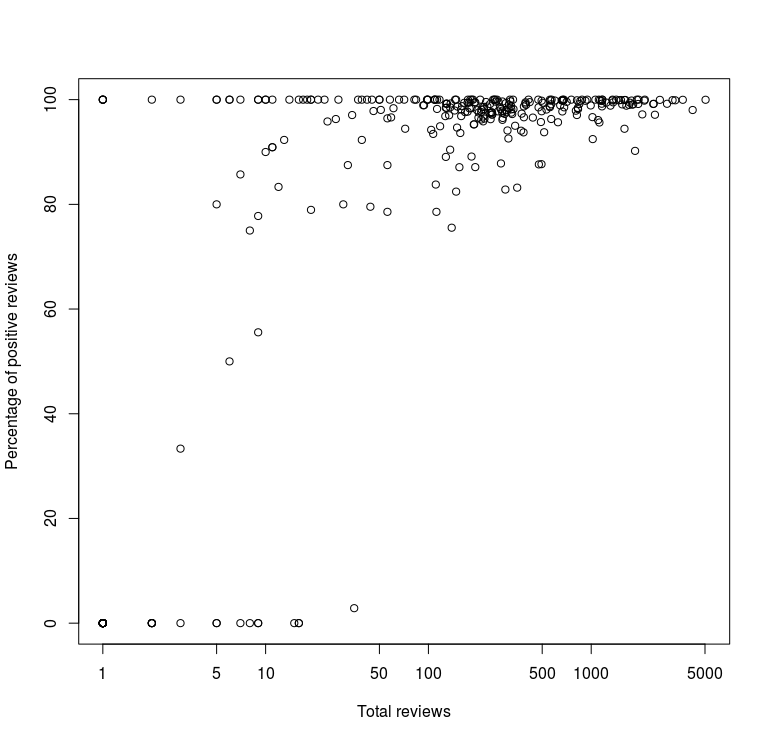
\includegraphics[scale=0.4]{pospercent}
    \caption{Positive reviews of vendors}
    \label{pospercent}
\end{figure}

\begin{figure}[!htb]
    \centering
    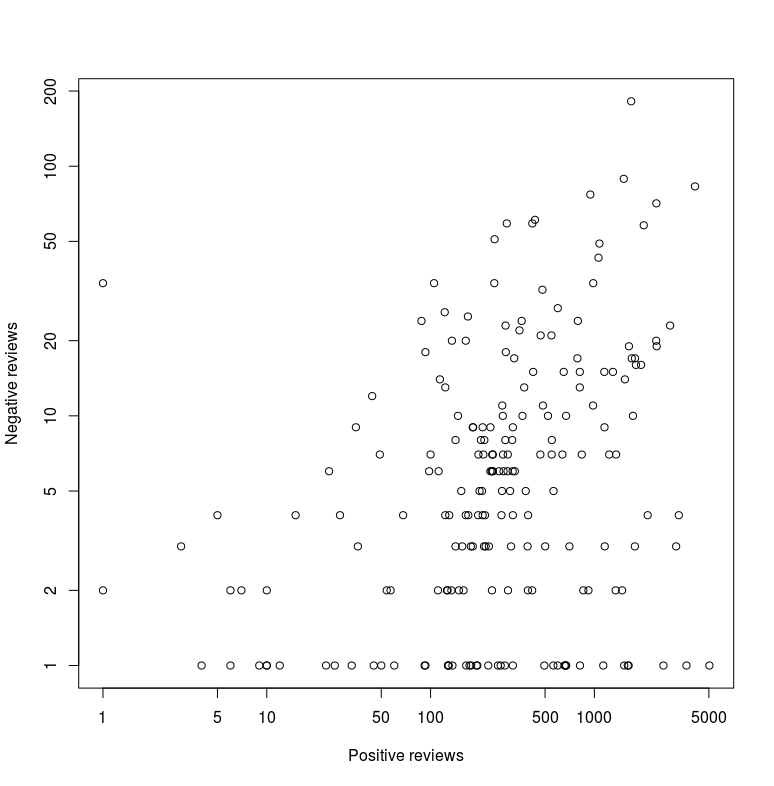
\includegraphics[scale=0.4]{posneg-log}
    \caption{Positive/negative reviews of vendors}
    \label{posneg}
\end{figure}
asfd
\begin{figure}[!htb]
    \centering
    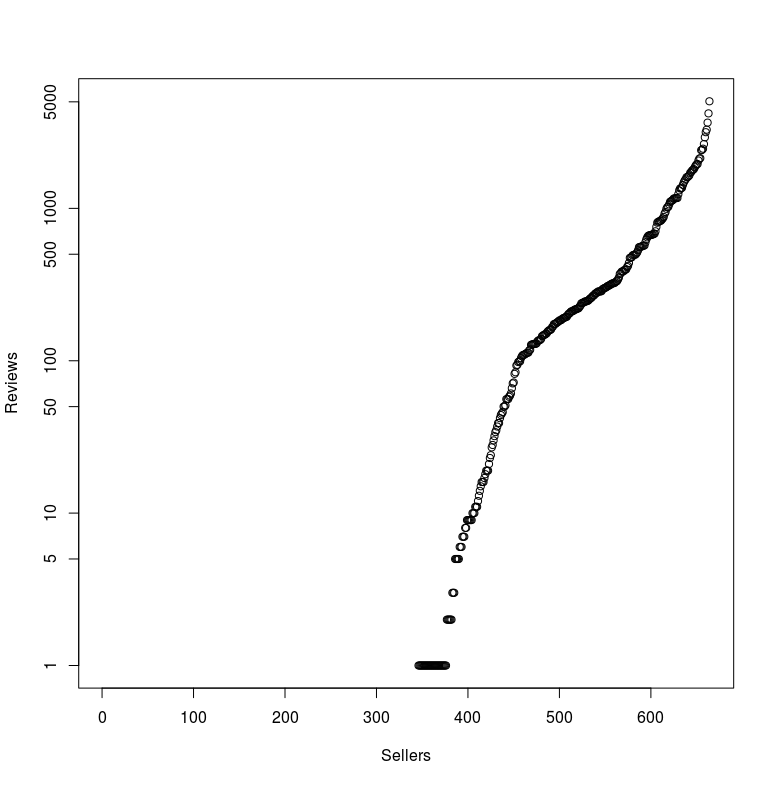
\includegraphics[scale=0.4]{reviews-count-log}
    \caption{Number of reviews for vendors}
    \label{reviews}
\end{figure}
asdf
\begin{figure}[!htb]
    \centering
    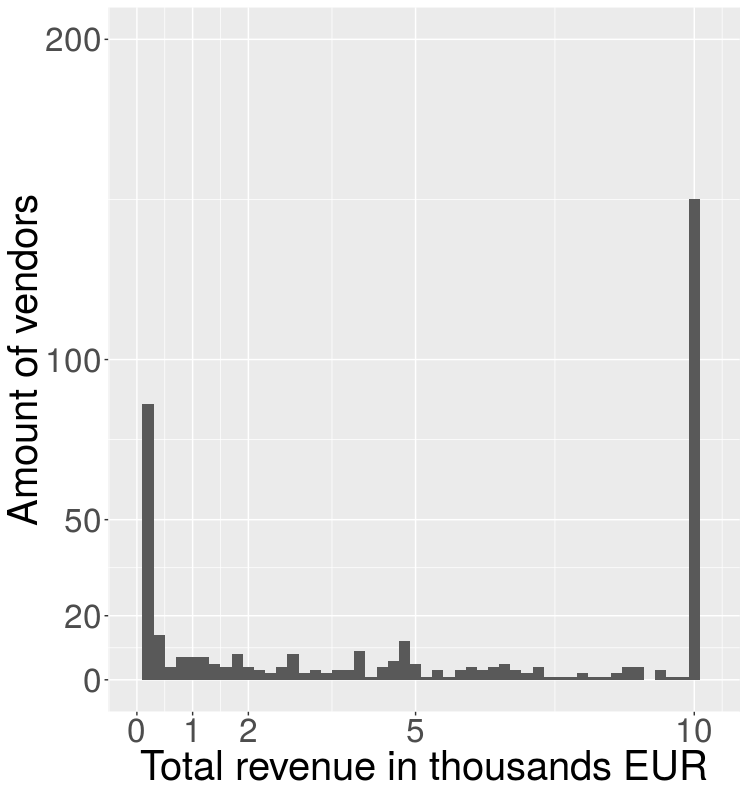
\includegraphics[scale=0.4]{total-rev}
    \caption{Total revenue of vendors}
    \label{Vendors by total revenue}
\end{figure}

\section{Statistics about vendors, drugs availability and distribution and buyers satisfaction}



\chapter{POC application}

This chapter describes the proof of concept application for investigating bitcoin address.
The application consists of three parts.
The scraping module, that downloads bitcoin blockchain and also scrape data from publicly available sites mention in section XXX.
The computanional module, which imports data to the database and also transform data. so that searching in these data would be fast.
The scraping, import and computanional modules are available for linux only.
The GUI written in HTML/JS/CSS, that is connecting to neo4j database REST endpoint and provides visualisation of data.
The GUI can be given a configuration string, to connect to neo4j REST API endpoint, so the gui can be viewed in broser from any device, as long as 
the server with neo4j data is reachable from that device.


\section{Implementation}

The importing module is responsible for parsing bitcoin blockchain files and importing the data into neo4j database.
The importing module take two parameters, the directory of .blk files, which store blockchain data and directory for creating neo4j graph database.
The import module firstly parses the .blk files and save blockchain as multiple .csv files. This intermidiary step is useful for debugging and also simplifies importing to neo4j database.

\begin{figure}[!htb]
    \centering
    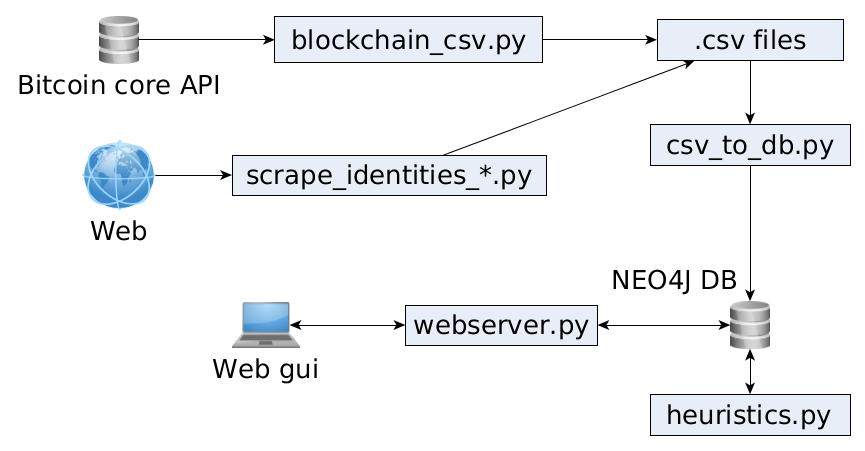
\includegraphics[width=1\textwidth]{application_architecture}
    \caption{Neo4j database ER diagram}
    \label{application_architecture}
\end{figure}

The next importing script is scrape\_identities.py script, which crawl popular forums and multiple websites and creates identities.csv.
File identities.csv contains 3 collumns.
\begin{itemize}
  \item Address - bitcoin address the identity is associated with
  \item Identity - String representing identity, usually username
  \item URL - Url where the Identity and Address were scraped
\end{itemize}

If the user has his own data about the owners of different bitcoin addresses, he can import it through the web GUI later.


\section{Usage}

\noindent See the following command :
\begin{lstlisting}[language=bash]
  $ ./import_module ~/.blockchain/ ~/neo4j/graph.db
\end{lstlisting}

\section{Future development possibilities}


\chapter{Testing and verification of the created tool}
This chapter describes the way, the POC application was tested.

The testing were performed by sending bitcoins to drug markets and withdrawing them.
Than marking the addresses from where the bitcoins were recieved as 

\section{Method of testing}
\section{results}



\chapter{Conclusion}

Here you can insert the appendices of your thesis.gg
\end{document}
